\documentclass{article}

\usepackage[%
    left=0.5in,%
    right=0.5in,%
    top=0.5in,%
    bottom=0.5in,%
]{geometry}%
\usepackage{minitoc}
\usepackage{multicol}
\usepackage{graphicx}
\usepackage{fixltx2e}
\usepackage{listings}
\usepackage{color}
\usepackage{hyperref}
    \hypersetup{ colorlinks = true, linkcolor = blue }
\usepackage{blindtext}
\definecolor{lightgray}{gray}{0.9}
\graphicspath{ {./} }

\newcommand{\inlinecode}[2]{\colorbox{lightgray}{\lstinline
[language=#1]$#2$}}
\newcommand{\worddef}[1]{\hyperref[sec:reference]{\textit{#1}}}

\begin{document}

\tableofcontents

\newpage

\section{Single core}
\begin{flushleft}
Each processor has a \textbf{private L1 cache}; it shares an \textbf{L2 cache} with its “chip-mate” and shares an \textbf{L3 cache} with the other processors.
\end{flushleft}
\begin{center}
  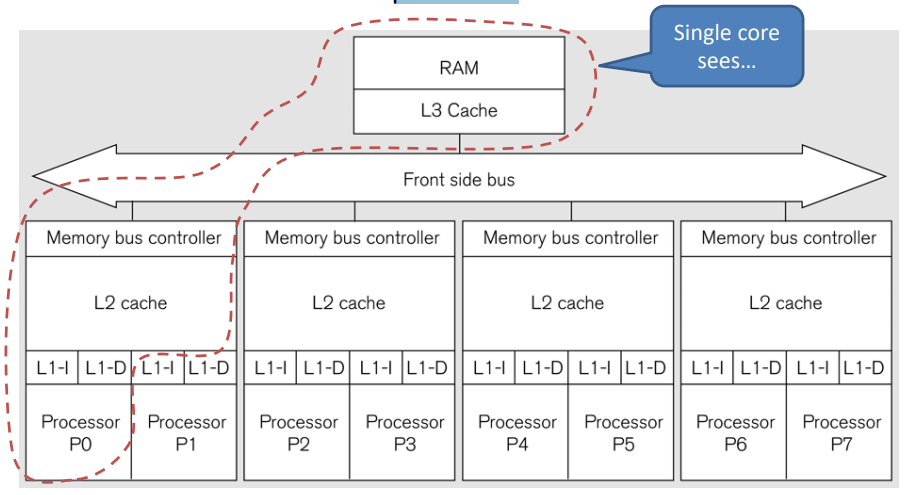
\includegraphics[scale=0.5]{multi_core_cache.png}
\end{center}

\subsection{Cache}
\begin{flushleft}
The purpose of cache memory is to store \textbf{program instructions and data} that are used repeatedly in the operation of programs or information that the CPU is likely to need next.
\\ \bigskip
\textbf{L1 cache}, or primary cache, is extremely fast but relatively small, and is usually embedded in the processor chip as CPU cache.
\\ \bigskip
L2 cache \textbf{may be embedded} on the CPU, or it can be \textbf{on a separate chip} or \textbf{coprocessor} and have a high-speed alternative system bus connecting the cache and CPU. That way it doesn't get slowed by traffic on the main system bus.
\\ \bigskip
L1 or L2 can be significantly faster than L3, though L3 is \textbf{usually double the speed of RAM}. With multicore processors, each core can have dedicated L1 and L2 cache, but they can share an L3 cache. If an L3 cache references an instruction, it is usually \textbf{elevated to a higher level} of cache.
\end{flushleft}

\pagebreak
\section*{Reference section} \label{sec:reference}
\begin{description}
	\item[placeholder] \hfill \\
\end{description}
\end{document}
